To generate valid switch states we developed two new algorithms. Both make
use of atomic islands.

\subsection{Random switch states through flooding}

The first method taken was implementing our own graph flooding algorithm that
produces valid partitions. A flooding method is well suited for the problem presented
as it starts at a node and expands out from there to connected nodes. This automatically
ensures that all nodes reached are connected. If the flooding starts at the 
transformer node, it is also ensured that the generated template contains a
transformer. To ensure that the entire graph is covered and that each template contains
exactly one transformer, flooding can be simultaneously started at each transformer.
To generate different switch states the choice of next node to flood to can be
randomized.\\
\\
Algorithmically this can be done by putting each node into its
own set initially.
Next a set of possible next options is formed by considering all neighbours of the
current node. One of them is then randomly chosen to be added to the set.
This process is then repeated until
all nodes have been added to one of the templates. 

\begin{algorithm}[h!]


    \SetKwFunction{GetRandomTemplates}{getRandomTemplates} % Define the function name
    \SetKwProg{Fn}{Function}{:}{} % Define the keyword and formatting
    \SetKwFunction{GetNextRandom}{getNextRandom}

    \Fn{\GetRandomTemplates{$edgesByNode$, $n$, $startingNodes$}}{

        \tcp{Initialize result templates with each of the initial nodes as the first element of the template}\label{alg:ssexp:random:init_templates}
        $templates \gets \{\}$\;

        \For{$n \in startingNodes$}{
            $templates \gets templates \cup \{n\}$\;
        }

        \tcp{Add nodes to templates until all of them have been visited}\label{alg:ssexp:random:main_loop}
        \While{$|visited| < n$}{

            \tcp{Determine what the next options for expansion for each template are}
            $next \gets \{\}$

            \For{$t \in templates$}{
                $currentNext \gets \{\}$\;
                \For{$node \in t$}{
                    \tcp{For each node in the current template add all neighbouring nodes as a next option, then remove all nodes that have already been visited}
                    $currentNext \gets  (currentNext \cup edgesByNode[node]) \setminus visited$\; 
                }
                $next \gets next \cup \{currentNext\}$\; 
            }

            \tcp{Choose a random template to update and a random node to add to that template out of the possible choices}\label{alg:ssexp:random:get_next}
            $templateChoice, \ nextNodeChoice \gets$ \GetNextRandom{$next$}\;
            
            \tcp{Update the chosen template and the overall visited nodes}
            $templates[templateChoice] \gets templates[templateChoice] \cup nextNodeChoice$\;

            $visited \gets visited \cup nextNodeChoice$\;

        }

        \KwRet $currentSets$\;
    }
    \caption{
        Flooding algorithm to obtain random switch state.
        $edgesByNode$ are the edges of the graph 
        in node representation (see eq. \ref{eq:graph_theory:node_form}),
        $n$ the total number of nodes and $startingNodes$ the node indices to start the flooding at.
    }
    \label{alg:ssexp:random}
\end{algorithm}

\autoref{alg:ssexp:random} outlines how such a random flooding algorithm may look like. The function \texttt{GetNextRandom}
is left as an external call here as changing how that choice is being made will have an effect on the generated template classes.
We have tried two approaches:

\begin{enumerate}
    \item Choose template to expand first, then choose node to expand
    \item Pick an expansion option out of all possible expansion options
\end{enumerate}

These are very different in the probability of which templates gets expanded
and thus the resulting template classes change in their distribution. Equations
\autoref{eq:ssexp:template_probability1} and \autoref{eq:ssexp:template_probability2}
show the probabilities of a template being expanded in any given iteration.

\begin{equation}
    p_{t, 1} = 
    \begin{cases}
        \frac{1}{|\{O_i \in O \ : \ |O_i| > 0\}|} & if \ |O_t| > 0\\
        0 & if \ |O_t| = 0
    \end{cases}
    \label{eq:ssexp:template_probability1}
\end{equation}

\begin{equation}
    p_{t, 2} = \frac{|O_t|}{\sum_{i=0}^{|T|} |O_i|}
    \label{eq:ssexp:template_probability2}
\end{equation}

where $T$ refers to the current set of templates and $O_i$ to the set
of current next expansion options for template $i$. In \autoref{eq:ssexp:template_probability1}
the probability for a template to expand is the same for each template, as long as there
are still expansion options. Meanwhile \autoref{eq:ssexp:template_probability2} implies that
a template is more likely to expand if it has more expansion options.\\
\\

\begin{figure}[H]
    \begin{subfigure}{.5\textwidth}
      \centering
      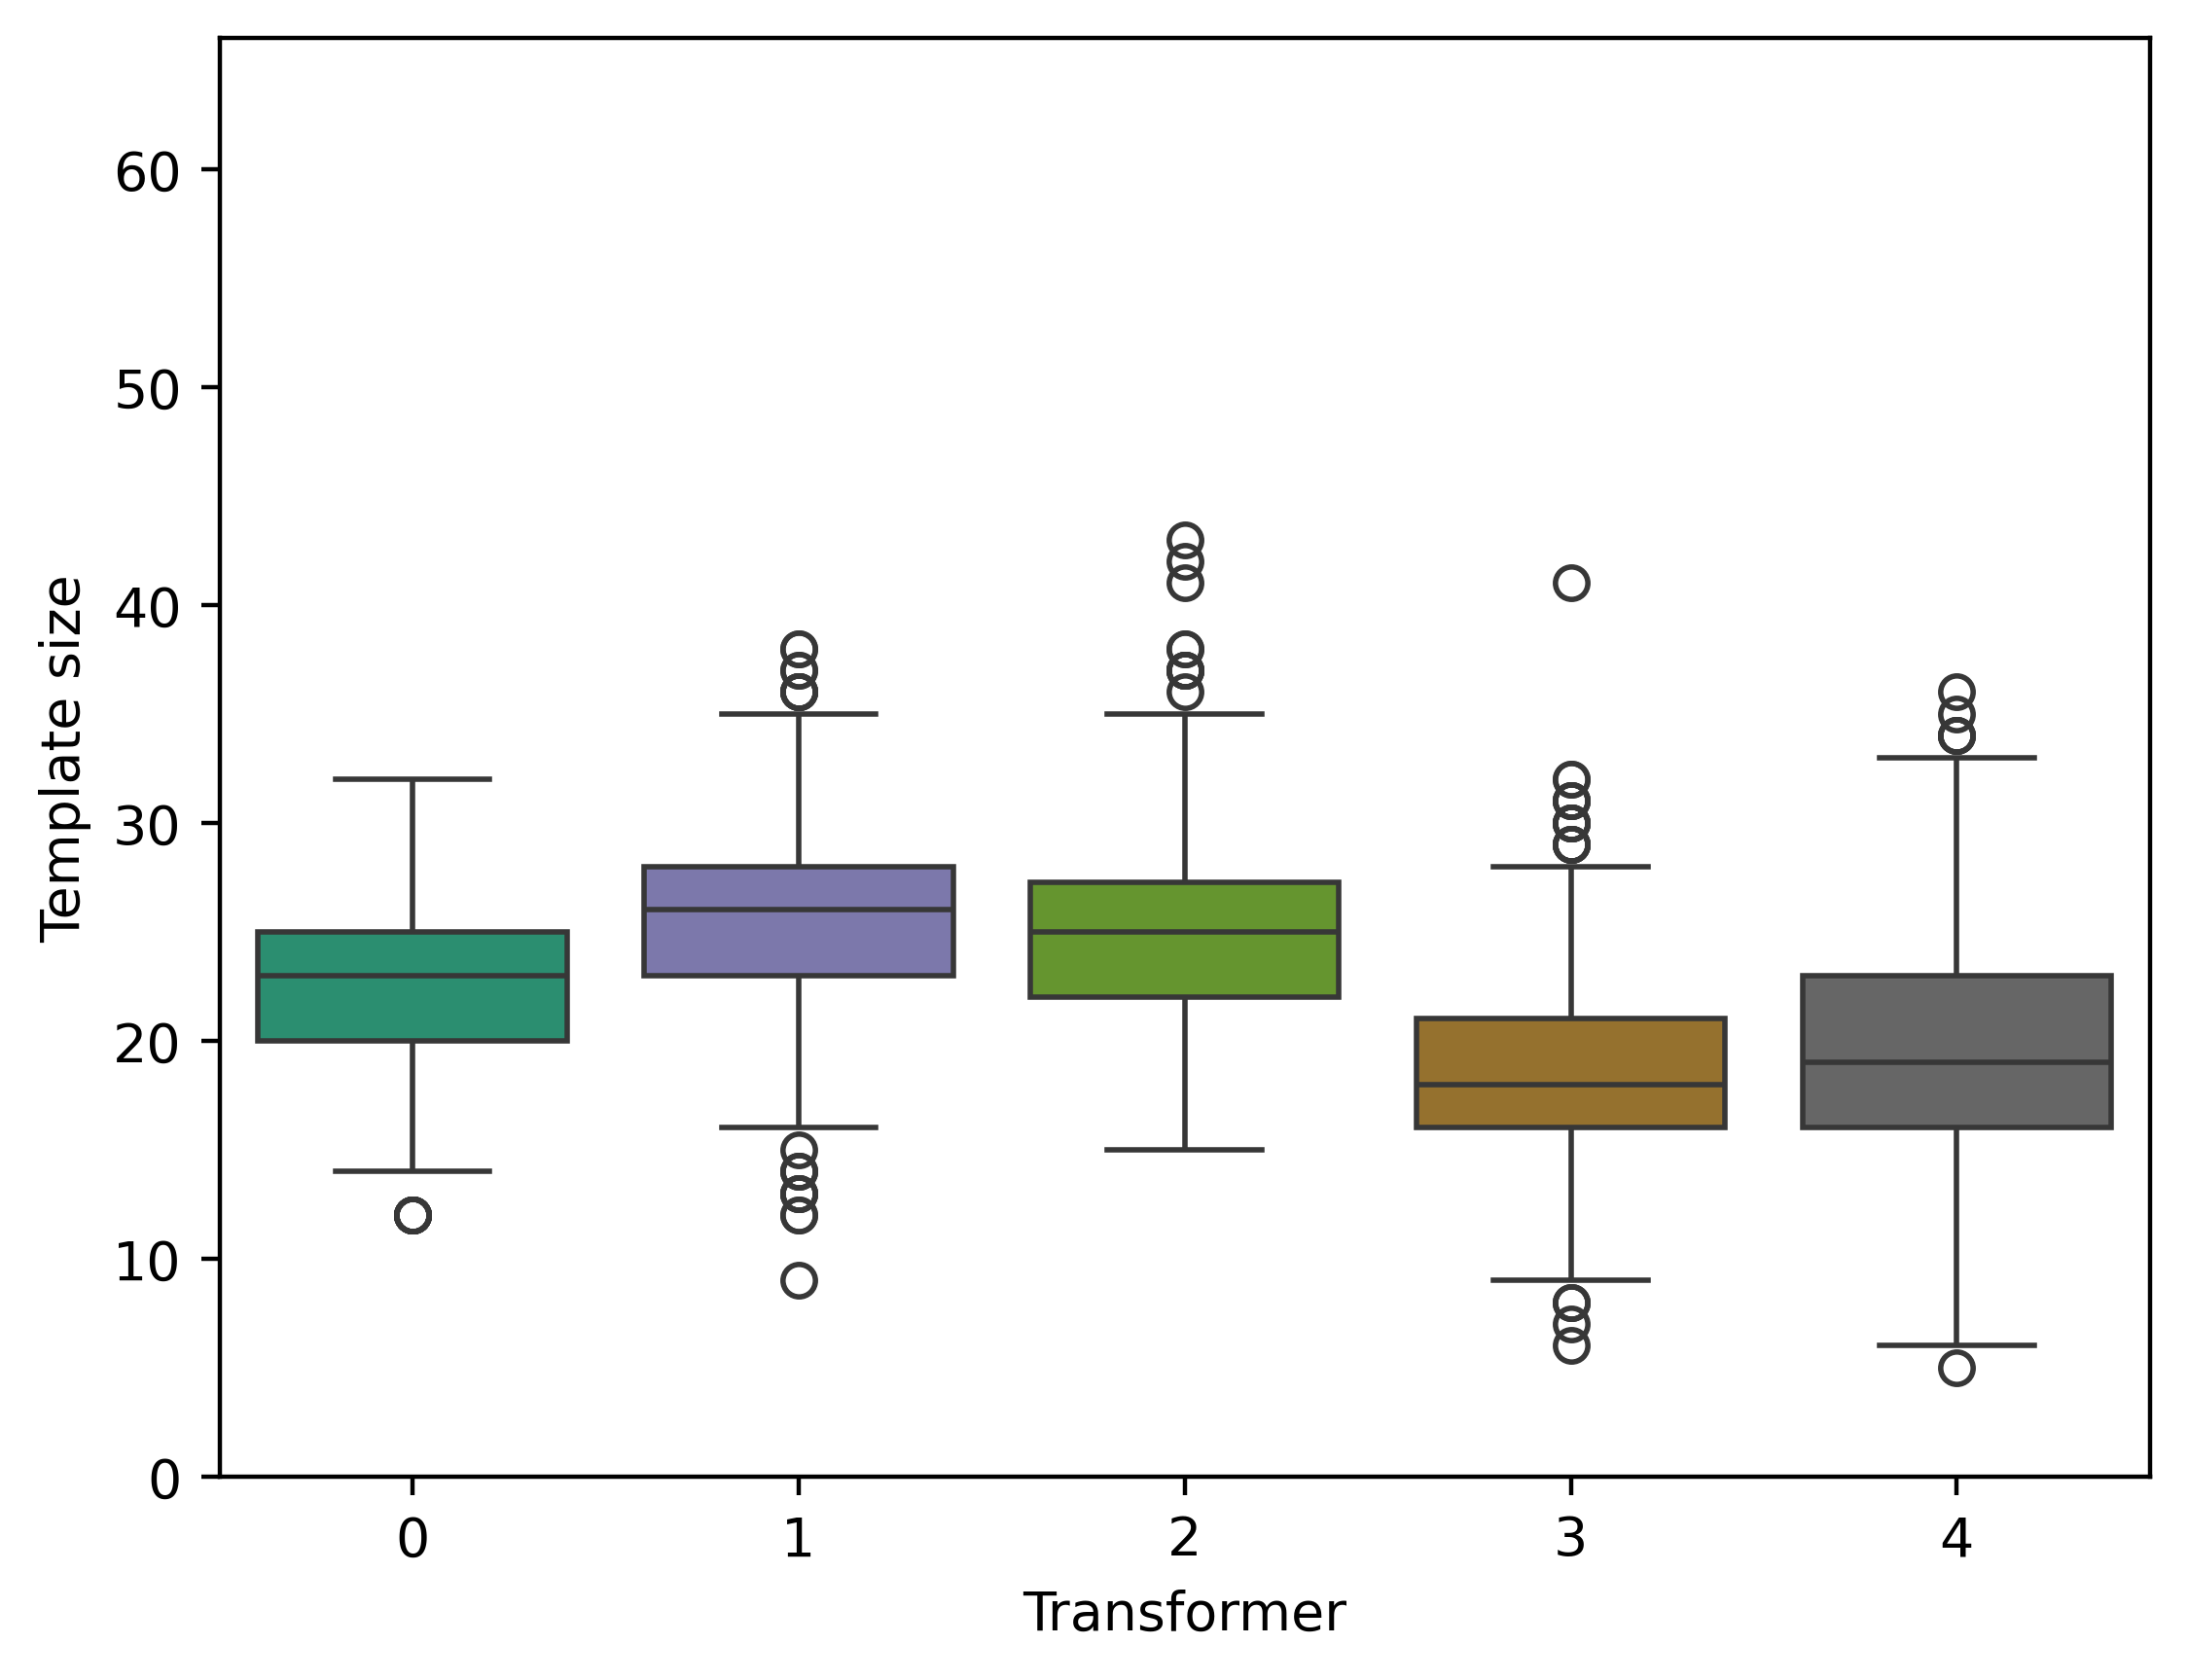
\includegraphics[width=\linewidth]{img/switchstate_exploring/swiss_suburb/random_switchstate_distribution_tempalte_p.png}
      \caption{}
      \label{fig:ssexp:switchstate_sampels_trafo_p}
    \end{subfigure}%
    \begin{subfigure}{.5\textwidth}
      \centering
      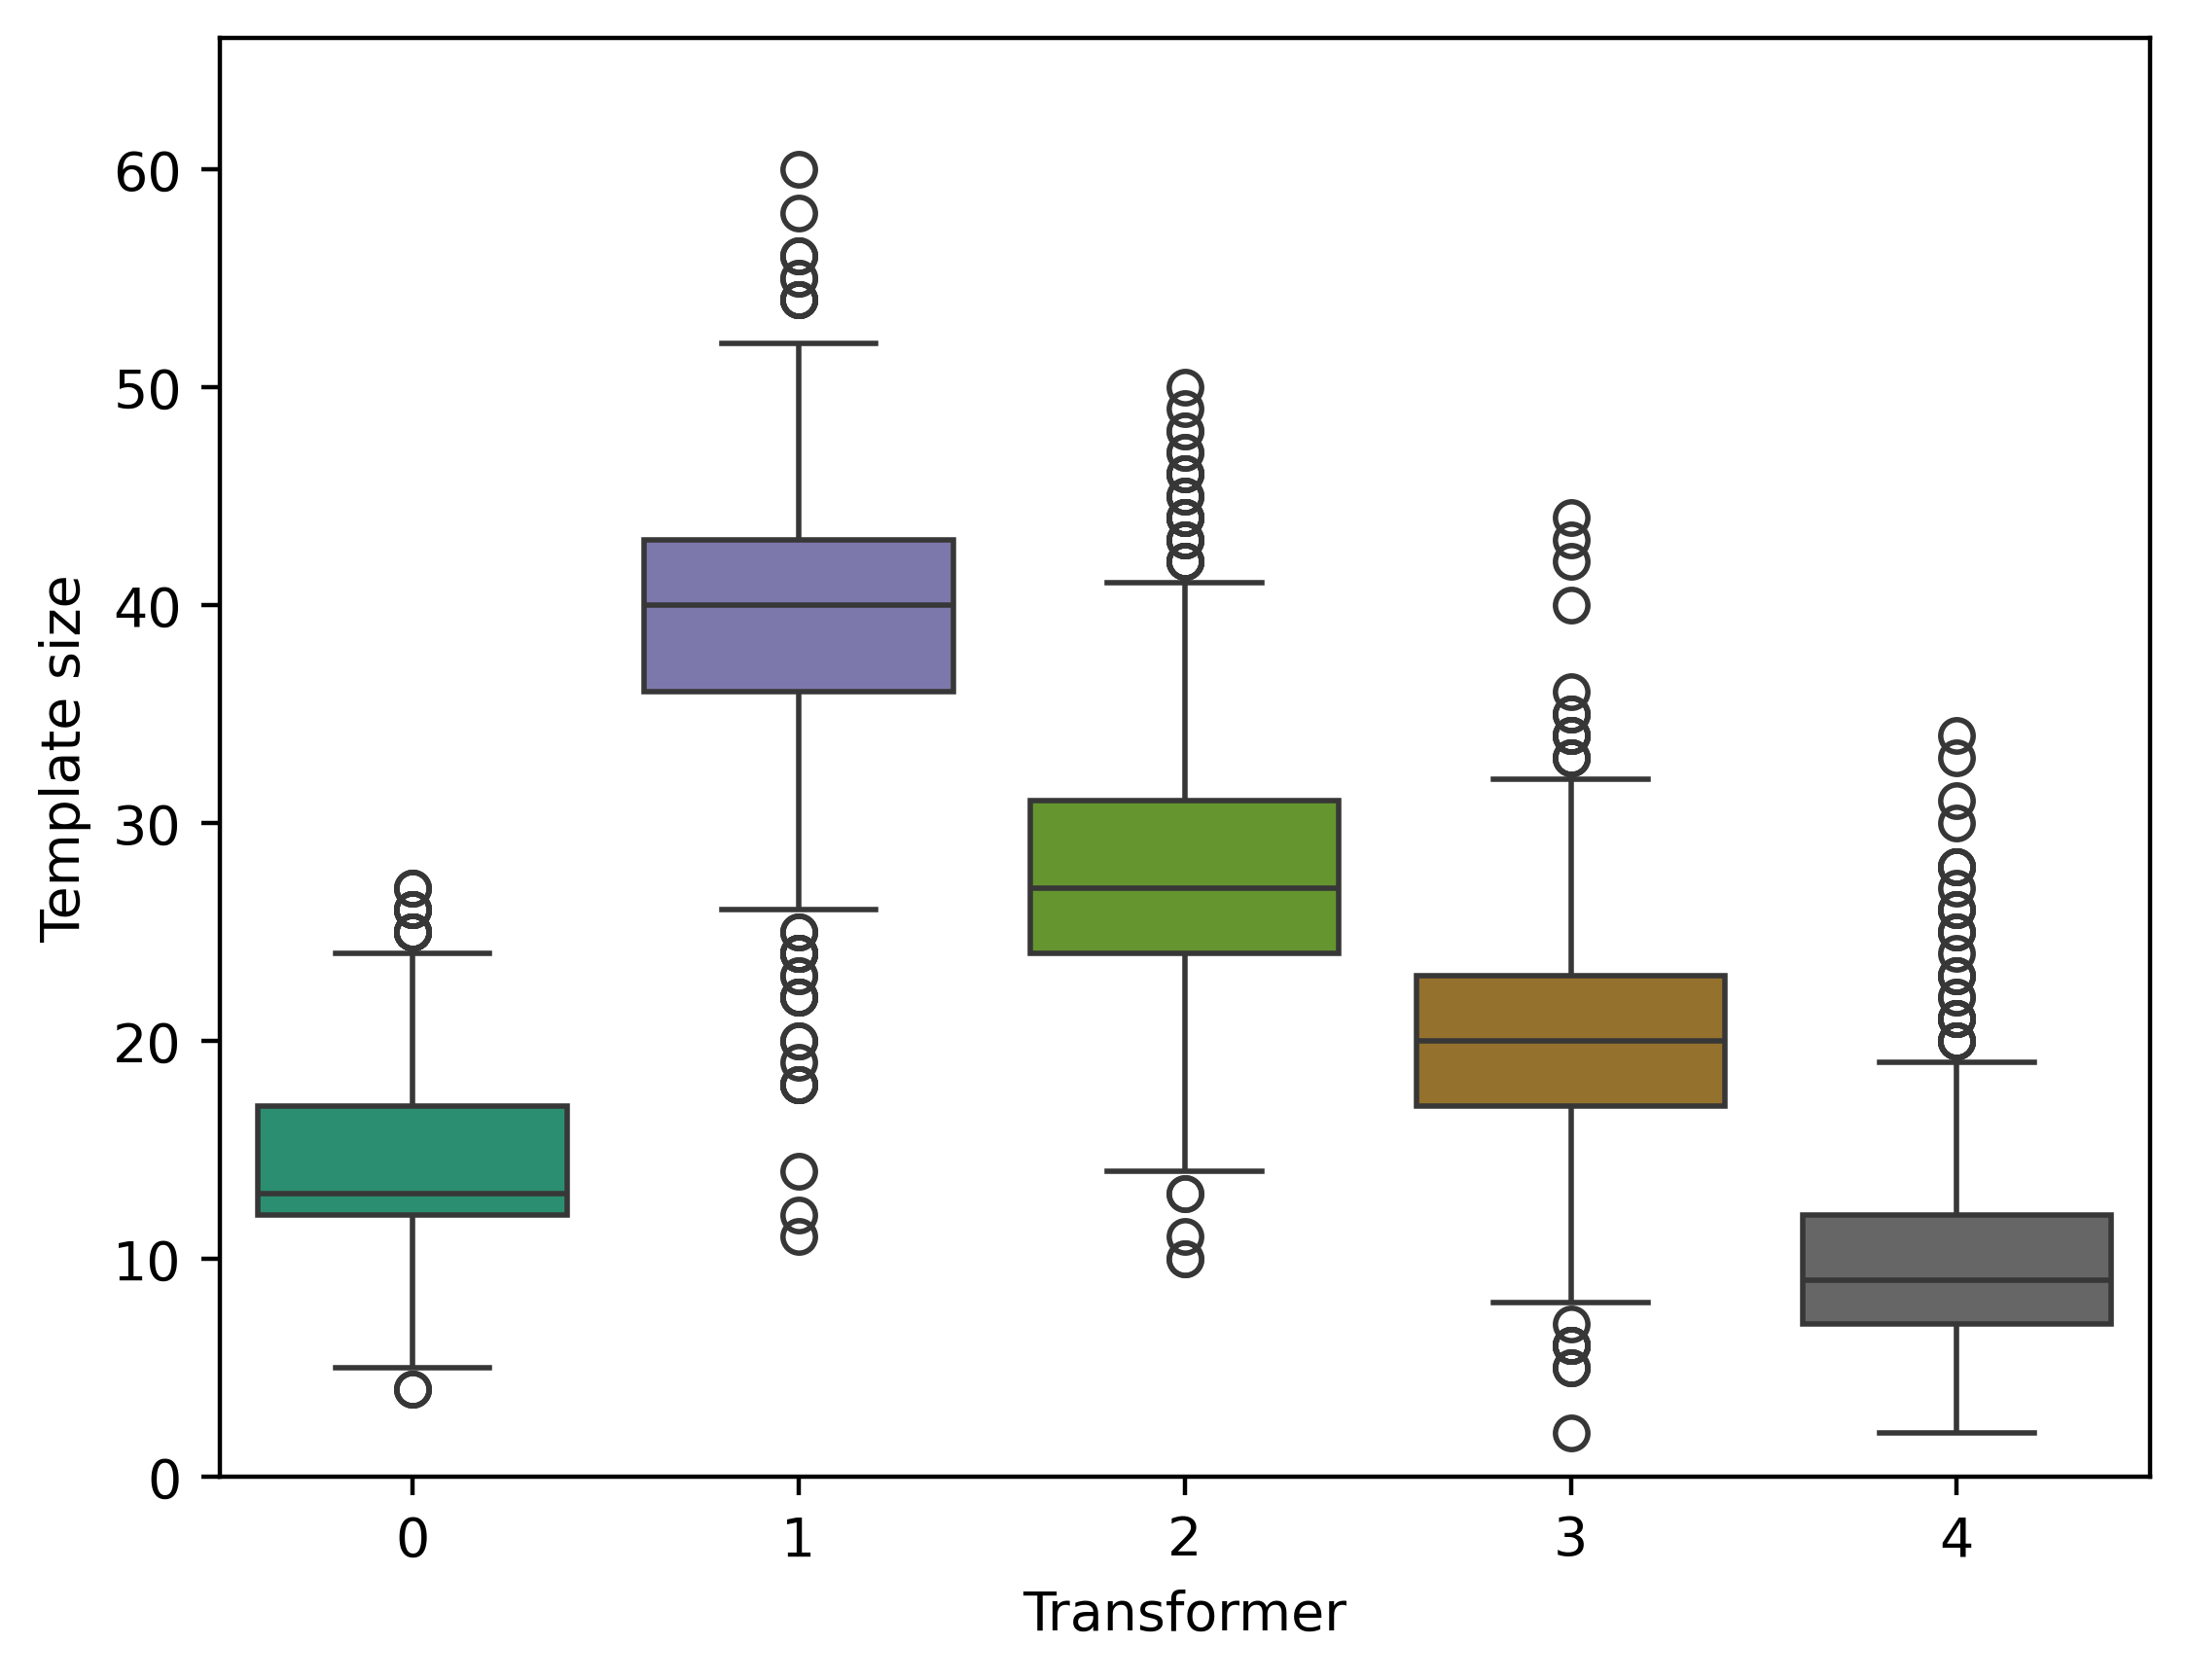
\includegraphics[width=\linewidth]{img/switchstate_exploring/swiss_suburb/random_switchstate_distribution_choice_p.png}
      \caption{}
      \label{fig:ssexp:switchstate_sampels_choice_p}
    \end{subfigure}
    \caption{
        Size of templates generated from \autoref{alg:ssexp:random}
        using \autoref{eq:ssexp:template_probability1} (a) 
        and \autoref{eq:ssexp:template_probability2} (b).
        Box plots showing the median, the 25\% quartile, the 75\% quartile and outliers used.
        1000 samples taken. Colours match template colours shown in
        \autoref{fig:data_prep:swiss_suburb_topology_patched}
    }
    \label{fig:ssexp:switchstate_sampels}
\end{figure}

\autoref{fig:ssexp:switchstate_sampels} shows the resulting template size
distributions when applying \autoref{alg:ssexp:random}. As expected, the
template sizes are more evenly distributed when 
using \autoref{eq:ssexp:template_probability1}
then when using \autoref{eq:ssexp:template_probability2}. 
Furthermore, templates generated using
\autoref{eq:ssexp:template_probability2} show a wider
spread of template sizes, whilst almost covering the full range
of sizes generated through \autoref{eq:ssexp:template_probability1}
(The exception being transformers 0, where the template 
never gets as large and transformer 1 where the template never 
gets as small).\\
\\
Due to these results \autoref{eq:ssexp:template_probability2} will
be used to generate switch state samples, as it should cover a wider
range of possible switch states.

\subsection{Random adjacent switch state}

Some optimization algorithms work by exploring neighbouring states
of an initial input state. To use these on the atomic island graphs
it is therefore useful to have an algorithm that returns a (random) 
new partition based on the current one. \autoref{alg:ssexp:adjacent}
returns a new partition with the exactly one atomic island changing
templates. 

\begin{algorithm}[H]
    
    \SetKwFunction{GetRandomAdjacentTemplates}{getRandomAdjacentTemplates} % Define the function name
    \SetKwFunction{Clone}{clone} % Define the function name
    \SetKwProg{Fn}{Function}{:}{} % Define the keyword and formatting
    \SetKwFunction{GetRandom}{getRandom}
    \SetKw{KwContinue}{continue}

    \Fn{\GetRandomAdjacentTemplates{$edgesByNode$, $templates$}}{

        \tcp{
            Make a list of all nodes that are on a template boundary
        }
        $possibleFlips \gets \{\}$\;
        \For{$template \in templates$}{
            $currentPossibleFlips \gets \{\}$\;
            \For{$node \in tempalte$}{
                $currentPossibleFlips \gets currentPossibleFlips \cup edgesByNode[node]$\;
            }
            $possibleFlips \gets possibleFlips \cup (currentPossibleFlips \setminus template)$\;
        }

        \While{true}{
            
            \tcp{Clone the templates to leave the old ones untouched}
            $newTemplates \gets$ \Clone{$templates$}\;

            \tcp{Get a random choice of template to enlarge and node to take from another template}
            $templateChoice,\ nodeChoice \gets$ \GetRandom{$possibleFlips$}\;

            \tcp{Update the chosen template with its new node}
            $newTemplates[templateChoice] \gets newTemplates[templateChoice] \cup \{nodeChoice\}$\;
            
            \tcp{Remove the node from its old template}
            \For{$tempalte \in newTemplates$}{
                $template \gets tempalte \setminus \{nodeChoice\}$\; 
            }

            \tcp{
                Check that each template is still valid, i.e. that it still
                has all nodes connected to each other. If not try another random choice
                }
            \For{$template \in newTemplates$}{

                $edges \gets \{\}$\;

                \For{$node \in template$}{
                    $edges \gets edges \cup ((i) \times edgesByNode[node])$
                }

                \If{$|$\GetConnectedIslands{$nodes$, $edges$}$| > 1$}{
                    \KwContinue \;
                }
            }

            
            \KwRet $newTemplates$\;
        }
    }
    \caption{
        Algorithm to get a random new partition with one node changing templates.
        $edgesByNode$ are the edges of the graph 
        in node representation (see eq. \ref{eq:graph_theory:node_form}),
        $teplates$ is an existing partition of a graph.
    }
    \label{alg:ssexp:adjacent}
\end{algorithm}

The method \texttt{getRandom} in \autoref{alg:ssexp:adjacent} works the same
as the \texttt{getNextRandom} in \autoref{alg:ssexp:random}. The probabilities
for a template to expand are similar as presented in equations \ref{eq:ssexp:template_probability1}
and \ref{eq:ssexp:template_probability1}, however $O_i$ instead refers to the number
of nodes connected to a template over an open switch or in other words nodes connected to a 
template belonging to a different template.
